\chapter{流式主题模型的参数结构}
\label{chapter:parameter}
参数服务器的出现,使得分布式并行算法的实现更加简便高效。
目前已知的大规模高效主题模型算法的实现都采用了参数服务器\cite{li2014scaling}, 
比如YahooLDA\cite{ahmed2012scalable}, LightLDA\cite{yuan2015lightlda}, 以及Peacock\cite{li2014scaling}(只实现了模型并行服务,还未抽象出来参数服务器)。
本章将介绍使用参数服务器来构建的流式主题参数数据结构,以及在此基础上的一些具体算法优化方案和参数备份和恢复机制。

\section{参数服务器简介}
\subsection{数据并行}
数据并行指的是将数据进行分割,并分配给不同的计算节点并行地执行计算任务。
提及数据并行,我们往往能够想到Hadoop MapReduce和Spark等系统。

MapReduce通过简单的Mapper和Reducer的抽象提供的编程模型,可以在一个由几十到上百台的廉价机器集群上并发地,分布式地处理海量数据集,同时具有高可用性。
Spark则是一种内存的MapReduce扩展,Spark的核心数据结构是RDD(Resilient Distributed Dataset, RDD),该数据结构可以将数据持久化在内存中,从而避免了MapReduce不同阶段之间数据需要反复落盘的缺点。

这些系统允许一些严格同步的通信和迭代。借助这些大数据并行计算框架,有人开发了一些基于数据并行的机器学习库,比如Mahout\cite{mahout}, MLI\cite{sparks2013mli}。
这些算法库在小规模算法上效果尚可,一旦集群规模变大或者算法模型变大,算法执行过程中的需要大量的网络通信以及参数同步,网络的延迟和漫长的同步等待,会逐渐影响算法执行速度。

\subsection{模型并行}
模型并行指的是将大规模参数模型分布式地存储在不同机器节点上,并行地利用所有数据训练算法。
在算法训练过程中,每个分区会得到一部分参数子集的更新,在最终更新到模型之前通常会各个分区的结果进行合并。
这种方法使用于具有大规模参数的模型,同时数据量又不是特别大的场景。
这种时候算法执行过程中不会频繁地进行网络通信,同时算法的每个分区只会使用和更新一小部分参数子集。这种方法的优点是,算法同步的效率高,网络通信开销和延迟小。但是当数据规模太大时,每个工作结点可能无法完全加载所有的数据样本。

\subsection{参数服务器}
在现实业务场景中,机器学习算法的数据量可能会非常之大,这使得单机无法完全加载训练数据,同时也无法存储下来所有的参数。
通常的解决方案是数据并行或是模型并行,这两种方案在一些场景中非常有用。
但是还有一些场景中,存在数据量和参数量都很大的情况,因而不得不同时使用数据并行和模型并行两种方案,但是同时应用这种两种方案往往使得程序的实现更加复杂,并且引入其他不稳定因素。

参数服务器的出现很好地解决了数据并行和模型并行同时应用的难的问题。
参数服务器使得数据并行过程中,算法可以在不同分区访问和更新全局参数(模型并行)。

\begin{table}\label{tab:jobs_failed} 
\center
\caption{某数据中心3个月机器学习任务统计}
\begin{tabular}{|r|r|r|}
\hline
$\approx$ \#machine $\times$ time & \# of jobs& failure rate \\
\hline
100 hours & 13,187 & $7.8\%$ \\
1,000 hours & 1366 & $13.7\%$ \\
10,000 hours & 77 & $24.7\%$ \\
\hline
\end{tabular}
\end{table}

论文\cite{li2014scaling}中统计了某数据中心3个月机器学习任务信息,表格显示随着算法规模的变大,任务出错的可能性也越大。

因而参数服务器主要解决如下挑战:

(1) 访问参数会消耗大量的网络带宽。

(2) 许多机器学习算法在并行过程中的许多步骤需要同步,这种同步很可能造成巨大的延迟。

(3) 当机器学习算法规模大时,系统越来越容易出错。


\begin{figure}[htb]\centering
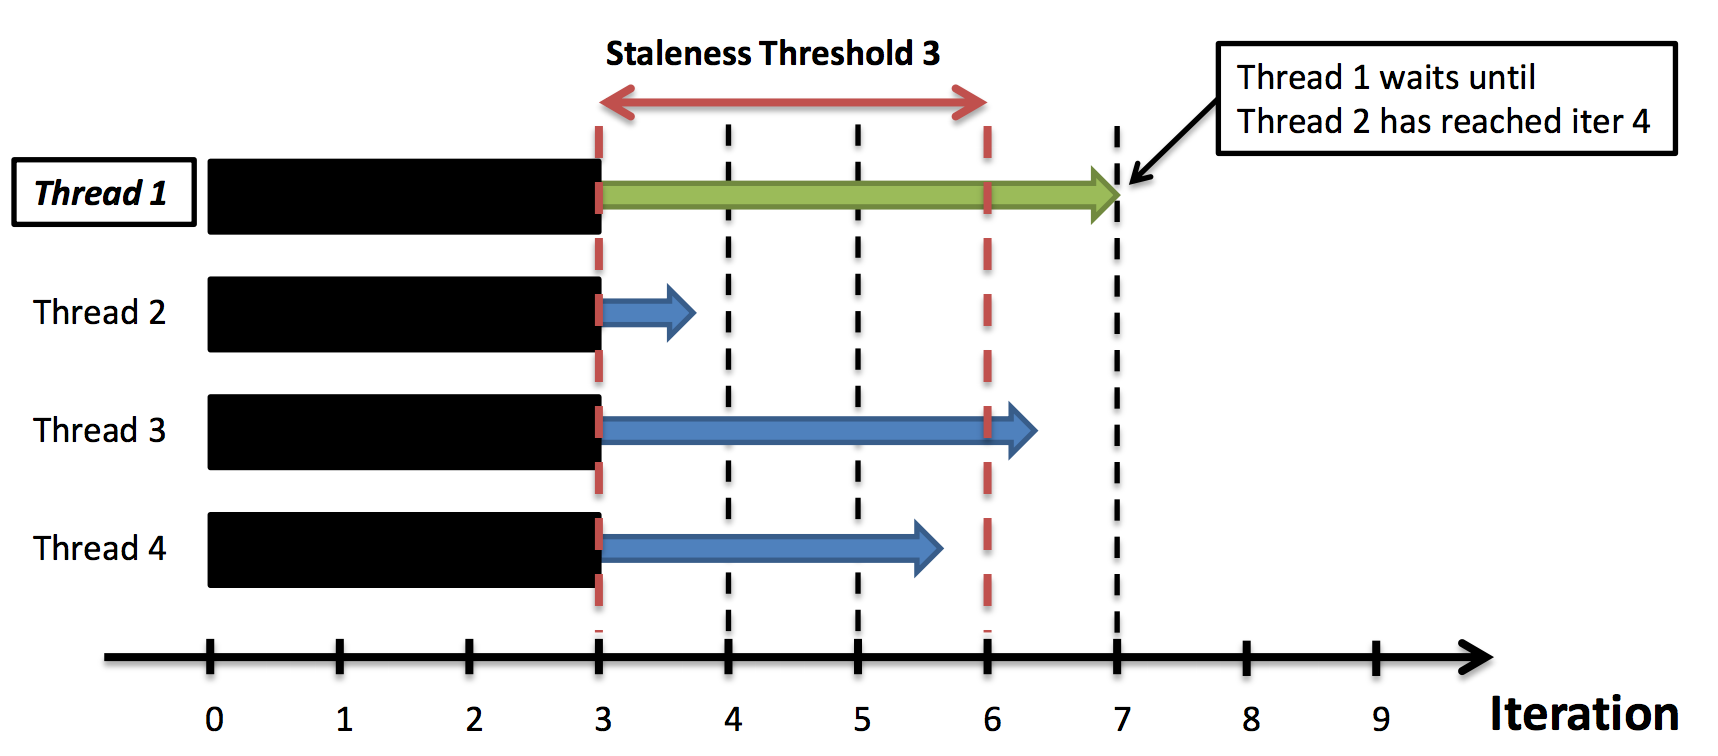
\includegraphics[width=0.8\linewidth]{SSP}
\caption{Stale Synchronous Parallel}
\label{fig:SSP}       % Give a unique label
\end{figure}

通常可以从两个方向着手缓解上述的挑战,第一个方向是通过更好的参数服务器实现和设计来提供更高效的服务;
另外一个方向是从算法应用的角度出发,通过更好的算法设计和参数服务器使用,来减少网络通讯和延迟。
前者的主要方式有压缩传输,Pipeline, SSP(Stale Synchronous Parallel, SSP)等等。
后者的主要方式包括从应用的角度减少参数的访问,使用更小更紧凑的参数类型,更稀疏的参数表示等等。为此,接下来本章将主要介绍如何设计分布式流式主题模型的参数存储和使用。


\section{参数结构的设计}
在互联网环境下,流式数据没有尽头,人们无法提前预知数据的分布,因而数据流上不断会有未登录词出现。
我们知道词汇的分布服从幂率分布,也就说大语料中绝大多数出现的词汇属于低频词,并且在流式数据中呈现出线性增长的趋势,如图\ref{fig:power-law, fig:noFreq2-5VsWords}。

\begin{figure}[htb]\centering
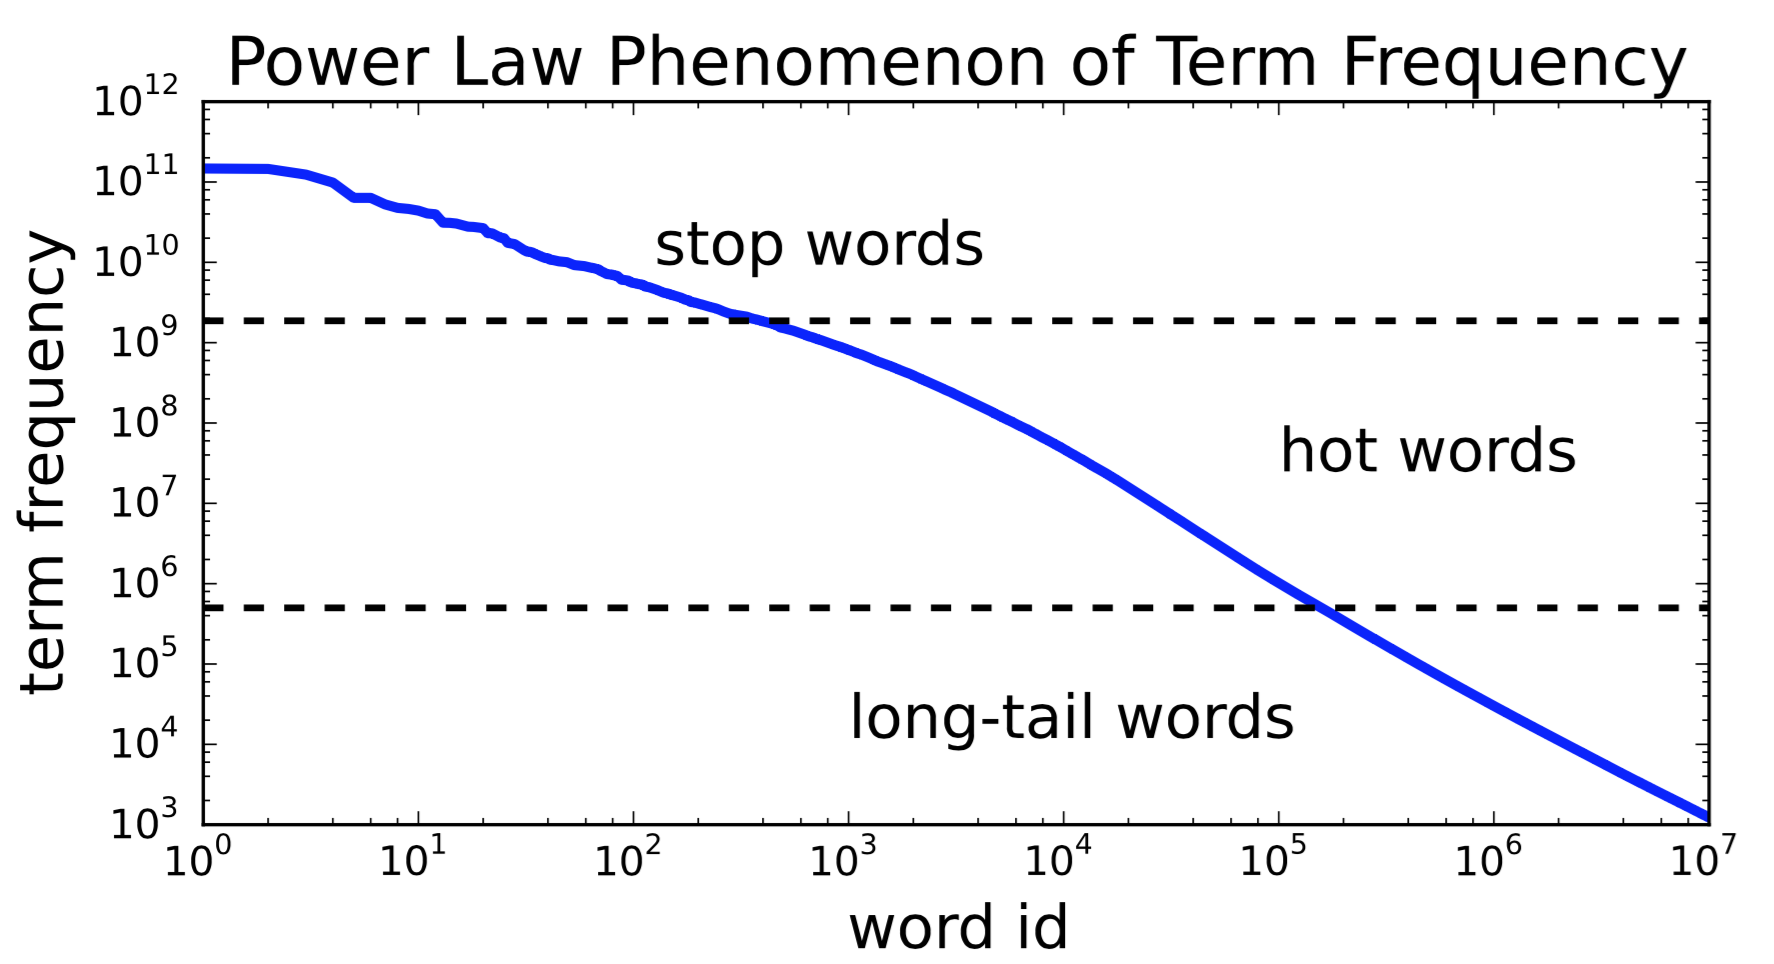
\includegraphics[width=0.5\linewidth]{power-law}
\caption{词频的幂率分布现象}
\label{fig:power-law}       % Give a unique label
\end{figure}

图\ref{fig:power-law}来自于论文\cite{yuan2015lightlda}, 是分析150亿个网页得到的结果,显示除了少量的静态词之外(几百上千),中间大约有几万-几十万个常用词,其他的词汇属于低频词。
论文\cite{yuan2015lightlda}还提到静态词和常用词大约只占所有词汇的$10\%$,而低频词却占了$90\%$。然而,静态词和常用词大约覆盖了$95\%$的语料,而低频词仅仅占了$5\%$。

\begin{figure}[htb]\centering
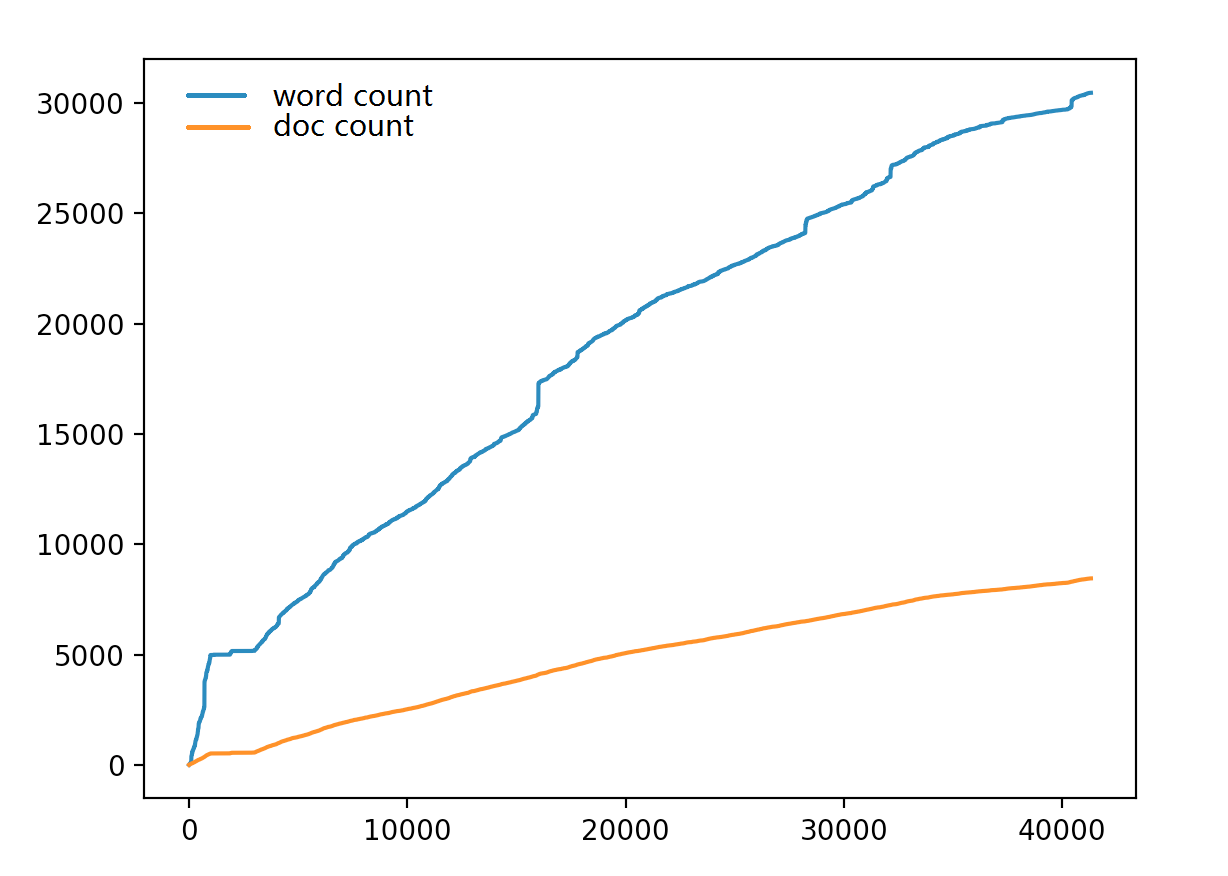
\includegraphics[width=0.5\linewidth]{noFreq2-5VsWords}
\caption{文档与低频词关系图}
\label{fig:noFreq2-5VsWords}       % Give a unique label
\end{figure}

图\ref{fig:noFreq2-5VsWords}中上方蓝色的线表示词频2-5的低频词随着文档数的增长趋势。下方的橙色线则表示包含这个区间内低频词的文档增长趋势。容易发现低频词的呈线性增长趋势。

通过前面章节的介绍,分布式主题模型的参数模型通常是一张词汇-主题计数表TAB(V, Z),表中的每一行对应着一个词汇的主题分布情况。在流式环境下,由于词表是动态增长的,这就意味着如果想要保留新增的词汇,那么我们必须维护一个动态词表。
因而维护一个动态词表的同时也要维护词汇-主题计数表TAB(V, Z)。
最简单的方式便是当词表中新增一个词汇时,相应地创建一个新的主题计数向量。
同理如果删除一个词汇也要相应地删除这个主题的计数向量。

根据上面的分析简单的动态词表维护策略,显然在实际应用中是行不通的。
这种做法将会遇到如下问题:

(1) 词表表超大,当主题个数超多时参数规模将会巨大无比。

(2) 维护动态词表,可能需要频繁的增删动态词表和词汇-主题计数表TAB(V, Z),这种维护代价有可能造成频繁的内存创建和回收,使得算法变得低效而无法被容忍。

解决和两个问题最为简单且行之有效的方法是使用先验知识提前设计一个静态的词表,这个词表里面只包含最经常被使用的一小部分词汇(根据前面的分析,仅需要涉及数十万个词汇即可)。
这种方法,避免了动态词表的维护,并且大大减少了参数规模,在许多主题模型的实现中都得到了应用。

\begin{figure}[htb]\centering
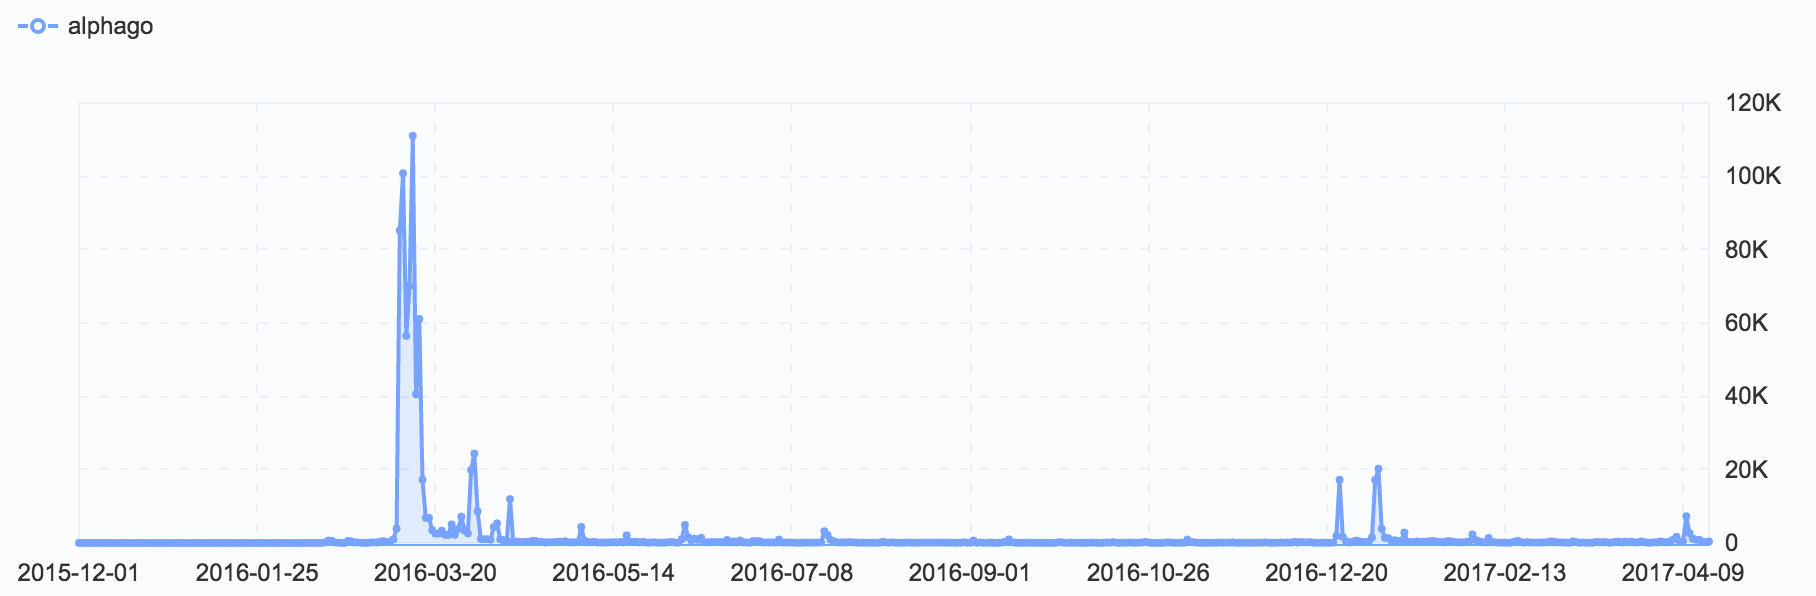
\includegraphics[height=0.23\linewidth,width=0.7\linewidth]{word-trend-alphago}
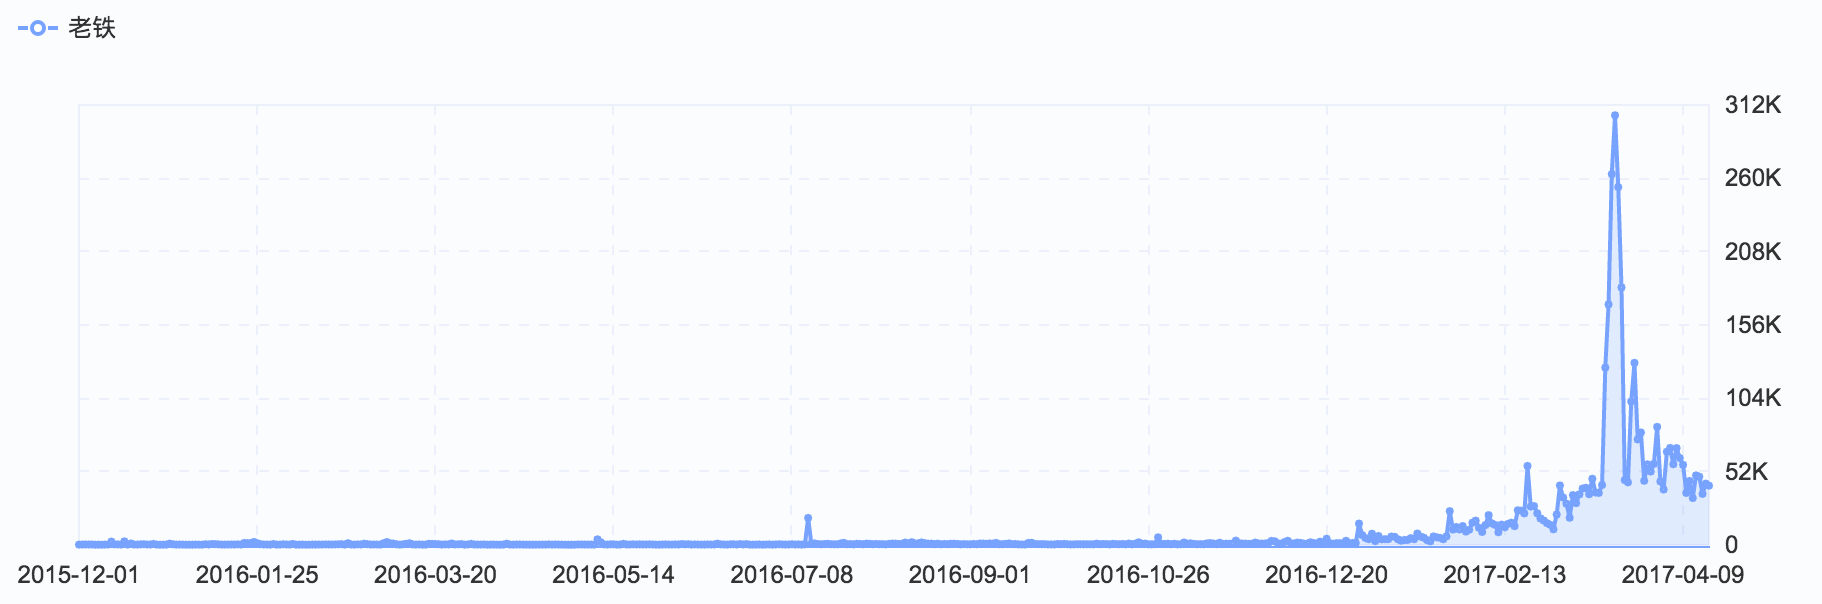
\includegraphics[height=0.23\linewidth,width=0.7\linewidth]{word-trend-laotie}
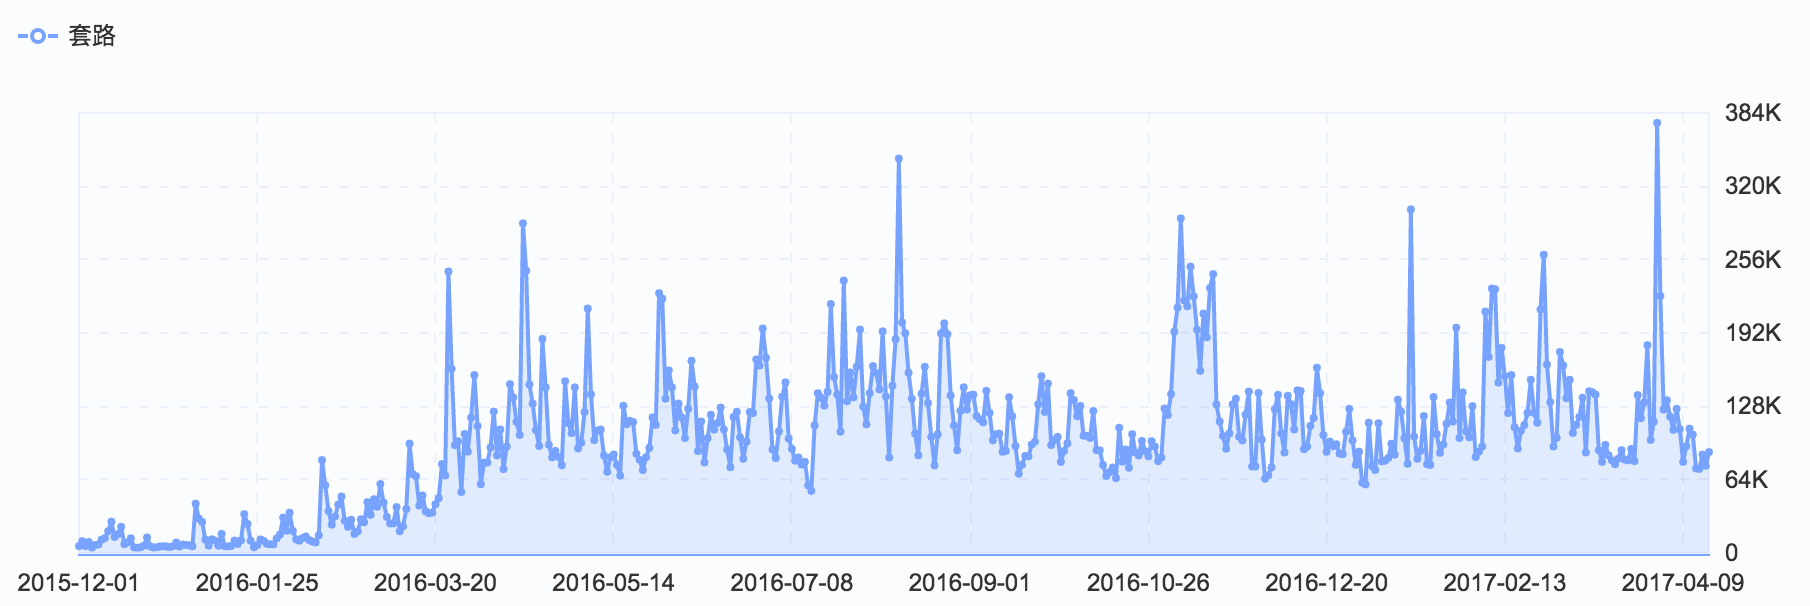
\includegraphics[height=0.23\linewidth,width=0.7\linewidth]{word-trend-taolu}
\caption{微博新词被提及的整体趋势}
\label{fig:new-word-trend}       % Give a unique label
\end{figure}

然而这种方法词表的规模很难确定,在不同的应用中主题模型可能需要不同阈值。
另外,固定大小的词汇表会使得许多有意义的词汇被忽略。
在流式数据中,由于词表是动态增长的,动态维护一个动态词表是有意义的。
因为社交网络的广泛应用和传播,使得许多新词被挖掘发现并得到追捧。图\ref{fig:new-word-trend}显示了今年来兴起的一些新词,类似的新词还有许多。

除此之外在具体的工业场景应用中,人们发现当数据量足够大且模型的主题个数足够多时,主题模型的效果会得到显著的提升。
这其中一个重要的原因是当数据量大时,许多覆盖低频词的主题语义被保留下来了\cite{Peacock}。
图\ref{fig:ntopics-pmi}显示了主题PMI分值,显然当主题个数越多时,PMI分值显著地提高了。

\begin{figure}[htb]\centering
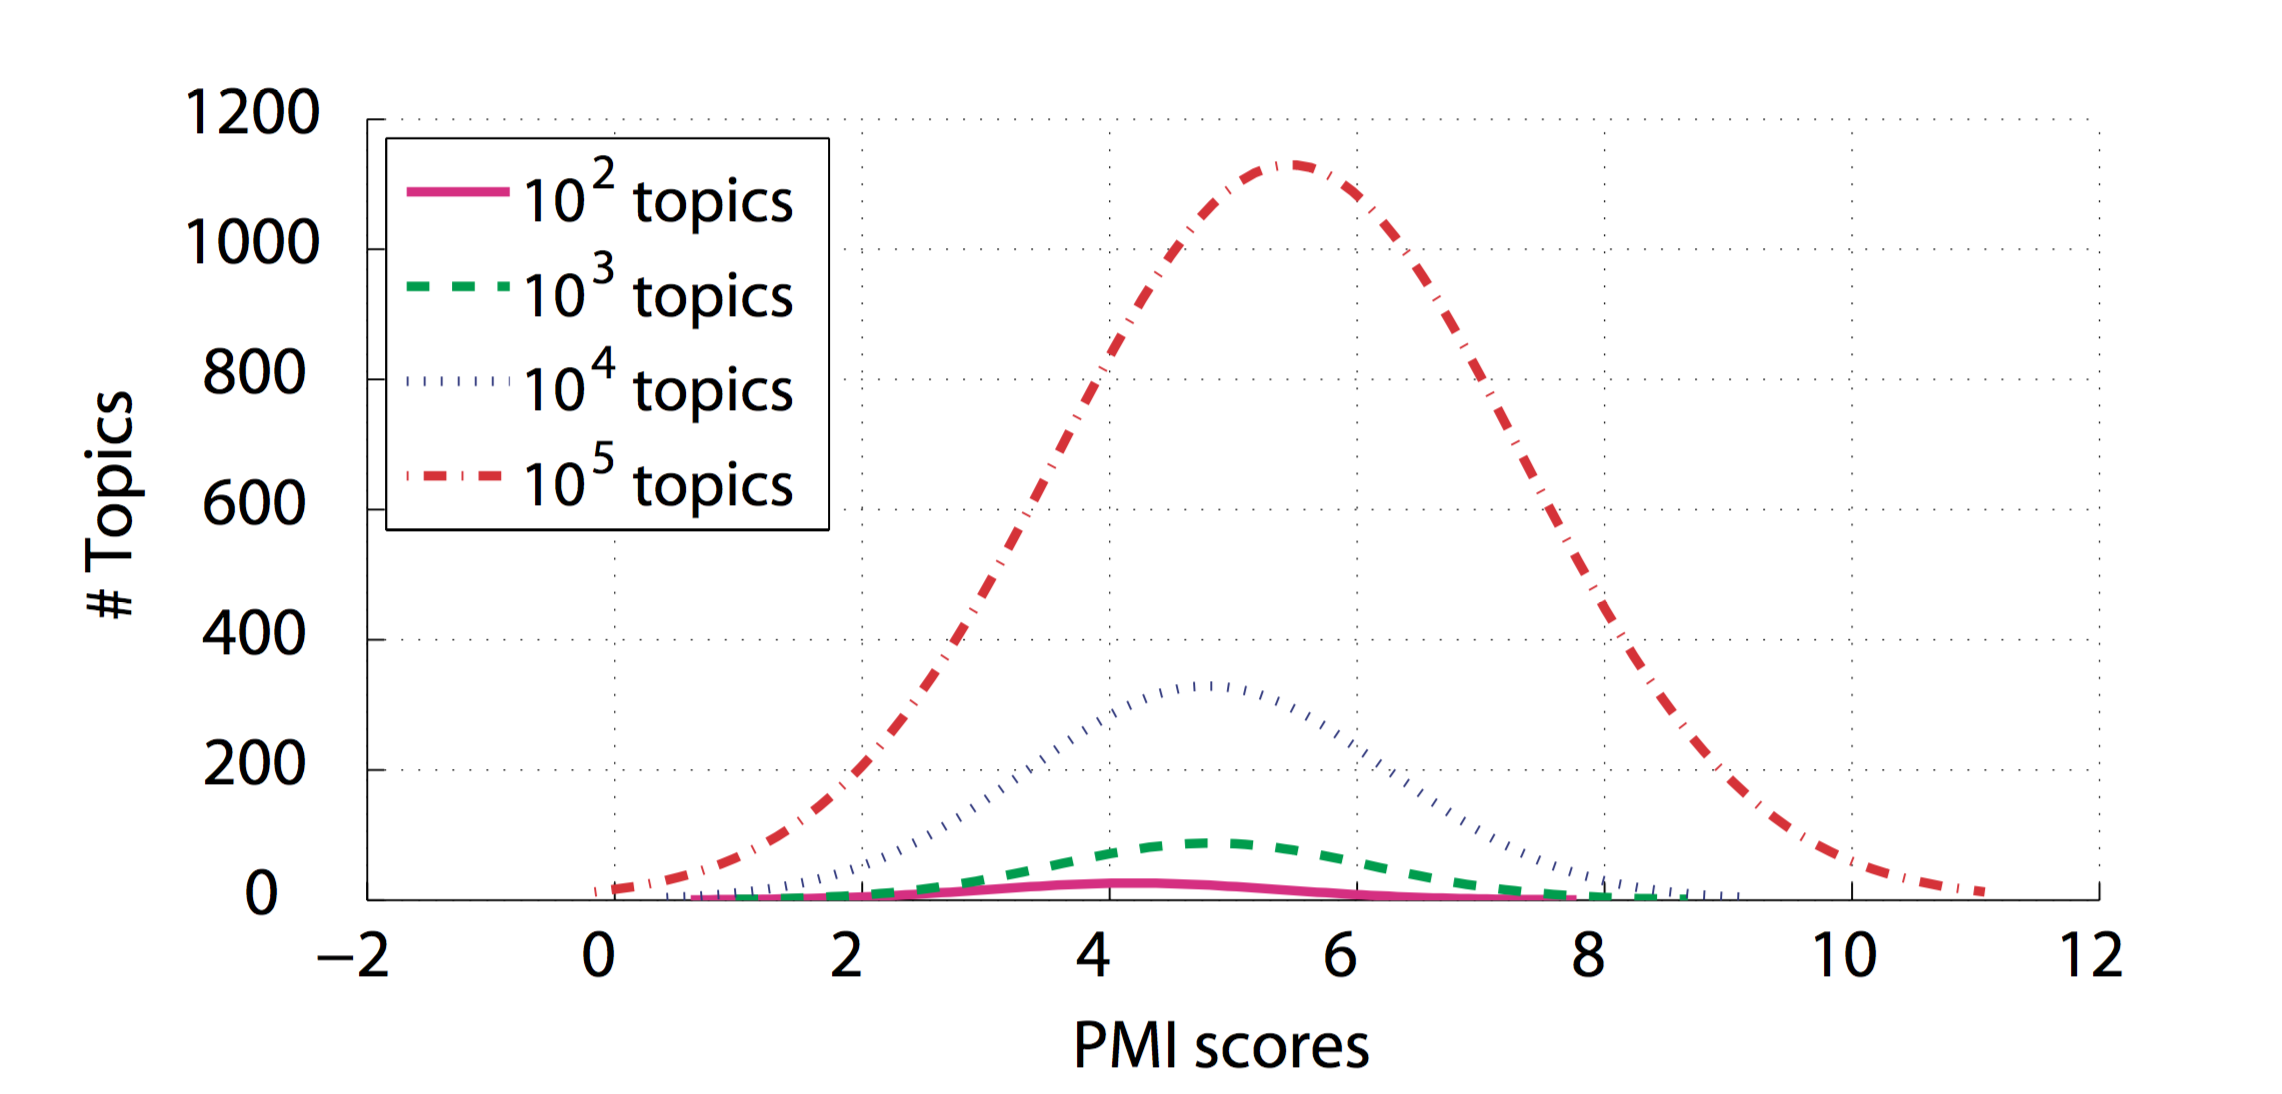
\includegraphics[width=0.7\linewidth]{ntopics-pmi}
\caption{LDA主题个数与PMI关系}
\label{fig:ntopics-pmi}       % Give a unique label
\end{figure}

这些分析都说明在流式数据上维护一个动态词表具有重要的意义。

实际上许多地方都提到了主题模型的词汇-主题表是一个特别稀疏的矩阵,对于大部分词汇来说,其语义是高度集中的,特别是低频词。
因而,如果采用稀疏表达的形式,比如哈希表,词汇-主题表的规模将大大减小。
然而完全使用稀疏表达也存在两个问题:

(1) 稀疏表达的矩阵或向量的随机访问效率不如稠密矩阵的高

(2) 当矩阵或向量相对稠密时,使用稀疏表达需要数倍于稠密的表达的空间消耗

上述的两个问题都会影响到主题模型算法的效率,其中第二个主要体现于在参数更新和访问过程中需要更多的网络传输。


\begin{figure}[htb]\centering
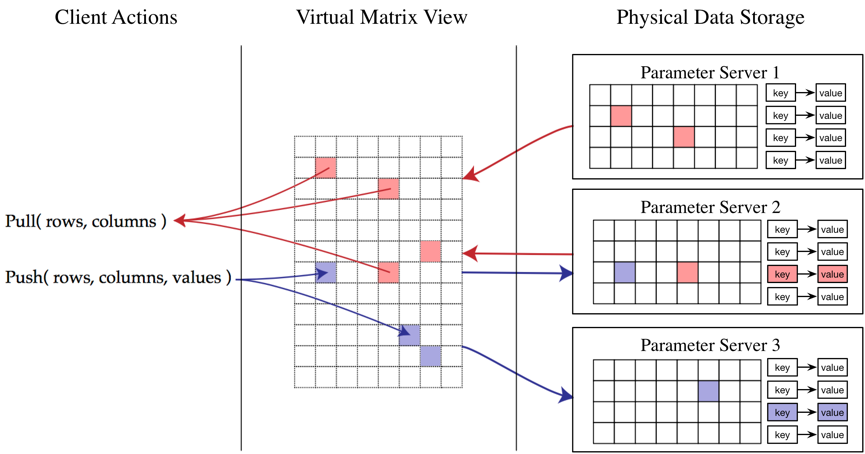
\includegraphics[width=0.8\linewidth]{hybrid-ps}
\caption{混合参数数据结构}
\label{fig:hybrid-ps}       % Give a unique label
\end{figure}

借助之前的分析结我们知道非低频词覆盖的数据大约占了$95\%$,也就是说在模型训练过程中有大量的参数访问来自于非低频词。
因而本文提出的解决方法是一种混合的参数数据结构。
这种混合数据结构既包含了稠密的表达,同时又包含了稀疏的表达。

在构建词汇表过程中,我们首先选取一个足够大的静态词汇表。
主要做法是选取一个相对较大的阈值筛选出了一部分高频词,针对这些词汇采用静态的词汇集表示,并构建<词汇, ID>映射。
剩余的词汇则采用动态的词汇表表示,由于数据流中不对会有新词出现,同时算法存在对过时的词汇的删除策略,因而动态词汇表时刻会产生变化。
所以,参数数据结构也会做出相应的修改。

如图\ref{fig:hybrid-ps},词汇-主题表所对应的参数结构按照词汇表的设计被划分成为了两个部分,其中一部分是静态的稠密矩阵表示,另外一部分则是使用<key, value>的形式进行稀疏的存储。

通过上面的设计方案,我们既高效地维护了一个动态词表,同时又使得绝大多数数参数访问和修改发生在了稠密矩阵上。

\section{参数数据结构的实现}
根据上面的参数数据结构的设计,在实现过程中我们还要考虑诸多因素。
在本文的实现中,我们使用了开源的glint\cite{glint}作为稠密参数的存储,使用了redis\cite{redis}内存键值缓存系统作为稀疏存储。
除此之外,在实现过程中我们还需要考虑到数值类型的选择,稀疏存储Sparse(V, Z)的稀疏性维护,参数系统的备份和恢复。

\subsection{使用int和float基本类型}
除了上面通过优化参数数据结构的方案来提高算法的参数服务器的使用性能之外,
一些具体的实现技巧也能大大提高算法的效率,这种思路在许多高效的算法实现中都能看到。

在基本类型中,最经常使用的整型int和浮点型float都只占用4个字节,而long和double类型通常占用8个字节。
这些类型的值域分别是:

int $\sim [-2147483648, 2147483647]$,

float $\sim [-3.4E(+/-)38, 3.4E(+/-)38]$, 

long $\sim [-9223372036854775808, 9223372036854775807]$,
	 
double $\sim [-1.7E(+/-)308, 1.7E(+/-)308]$。

int和float所能表示的范围和精度有限,当数据太大时可能造成溢出。
然而当参数规模足够大时,使用4字节类型和使用8字节类型之间将会有成倍的存储效率差距。

但是根据图\ref{fig:power-law}显示,除了静态词很少会有词汇超过int所能表达的值域。而在主题模型中静态词通常会在训练之前被遭到过滤。因而如果使用long和double类型意味着很大的浪费。

在本文的实现中,我们选择了4字节基本类型作为参数类型。


\subsection{稀疏存储Sparse(V, Z)的维护}
在本文主题模型参数数据结构的设计中,低频词-主题分布表Sparse(V, Z)的稀疏性起到了至关重要的作用。
但是如果没有得到维护,也会显现出一些问题。本节主要介绍流式环境下如何维护Sparse(V, Z)稀疏矩阵。

在上一章,本文介绍了两个流式主题模型算法框架,分别是在线流式主题模型\ref{alg:onlineStreamLDA}和增量流式主题模型\ref{alg:IncStreamLDA}。

实际上在线流式主题模型中,参数$\beta^{(t)}(w, k) = (1 - \rho_t) \beta^{(t-1)}(w, k) + \rho_t n_{k, w}^{(t)}$是一个加权平均值。其中$\rho_t \in (0, 1)$,说明几轮迭代之后,$\beta^{(t)}(w, k)$将会出现很多小数值。
假设$\beta^{(t-\sigma)}(w, k) = 1$,并且在其后的$\sigma$轮迭代中都有$n_{k,w} = 0$,
那么$\beta^{(t)}(w, k) = (1 - \rho_t)^{\sigma} > 0 $。
我们发现$\beta^{(t)}(w, k)$将会变得较小,但是不会变为0。
换句话说,$\beta^{(t)}$矩阵中将会出现大量的非零元,Sparse(V, Z)的稀疏性会大大降低,带来的是存储空间的消耗和更多的网络传输。

然而$\beta^{(t)}$中的绝大多数非零元对LDA Gibbs采样概率分布的影响微乎其微。
为了保证$\beta^{(t)}$的稀疏性,本文提出了两种做法:

(1) 设置阈值,对较小的小数进行截断。比如,如果$\beta^{(t)}(w, k) < 0.05$,删除该非零元。

(2) 采用int类型存储$\beta^{(t)}$,在每轮迭代的执行加权平均时使用四舍五入的方法转为整型。

相对于在线流式主题模型,增量主题模型只有增量的更新操作,并且每次更新都是一个整型值,所以更适合于参数服务器的使用模式(增量地更新)。
另外,因为增量流式主题模型设置了窗口大小,所以模型中参数值$\beta(w, k)$最终稳定在某一个范围区间内。
同时,随着模型的逐渐收敛,$\beta^{(t)}$中的元素会出现越来越多的零元。

以上两个算法都需要单独的步骤来删除稀疏数据结构Sparse(V, Z)中的零元来提高非零元的存储比例,减少不必要的网络传输。

\subsection{参数的备份和恢复}
前面已经介绍了在对于一个长时间运行的系统,任务失败是一个很常见的事情。
造成这些错误的原因多种多样,在流式主题模型中主要的原因可能有:
(a) 程序内部的BUG;(b) 算法运行超时;(c) 网络拥塞造成节点通信失败。

现有的分布式并行处理框架都有设计并提供容灾机制。
比如Spark中,如果一个Task失败之后,任务调度器还会尝试重启运行改Task。
本文的流式主题模型就是在Spark Streaming的计算框架下实现的。

然而Spark所提供的容灾机制并不能解决本文所提出的流式主题模型失败的问题。
主要原因在于,在流式主题模型运行采样过程中,算法会频繁地更新参数服务器上的参数。
虽然我们引入了许多优化方法,降低了模型参数的同步要求提高了并行度,但是在算法执行过程中参数服务骑上的参数始终维持一致性。
当错误出现时,部分参数将会丢失,系统会抛出任务失败信息,但是我们无法定位失败时程序执行的位置。
也就是说,参数服务器上的参数一致性受到了破坏。
在这种情况下,即使我们重启了Task,仍然无法恢复参数的一致性,因而继续执行算法仍然会持续失败。

为了提升算法系统的可用性,本文设计了参数的备份和恢复机制,如图\ref{fig:recovery}。
\begin{figure}[htb]\centering
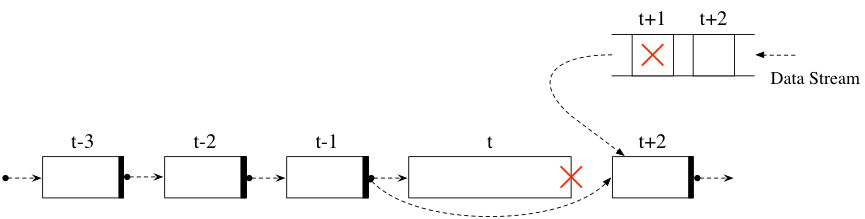
\includegraphics[width=1\linewidth]{recovery}
\caption{备份和恢复机制示意}
\label{fig:recovery}% Give a unique label
\end{figure}

\subsubsection{备份机制}
在本文的算法设计中,算法的参数在某些时刻是维持同步的,这些时刻包括每轮迭代之前和迭代完成之后的时刻。
虽然这些时刻都可以作为合理的参数被份节点,但是本文的算法实现中我们选择了流式数据每个时间片开始执行之前的时间节点作为参数备份节点。

我们知道,参数的备份是一个耗时耗空间的操作,并且在备份期间算法无法算法必须停止运行。
但是,为了维护系统的稳定性保证在失败时能够正确地重启算法,备份机制是必要的。
考虑到这些因素,流式数据的自然时间切片是一个较好的备份时间间隔。
在图\ref{fig:recovery}中每个时间片执行完成之后便会启动备份,虚线箭头左端的黑色区域表示备份阶段。
下一个时间片的算法之前参数需要与备份的参数保持一致。
这么做我们不仅能够更好地维持流式数据的动态变化模型,而且使得算法系统花在备份的时间空间相对较少。

\subsubsection{恢复机制}
根据前面的叙述,算法运行超时是算法执行失败的一个重要因素。
在真是应用场景中,由于流式数据的突发性特点,每个时间片的每个分区的算法运行时间很难得到有效的控制。
所以,超时是一个时常发生的事情。尽管如此,也并不是所有的超时都会引起失败。
那些引起失败的时间任务势必严重超时了。

在算法失败之后,为了保证系统继续运行,必须引入算法的恢复机制。
然而恢复机制的选择对系统的稳定性也有较大的影响。
一方面恢复是一个耗废资源的操作,并且在此期间算法也要停止运行;
另外一方面,即使正常恢复了算法运行,不同的恢复机制也对算法继续运行的鲁棒性有影响。

在前面提到的超时失败的问题中,如果算法直接从失败的位置恢复并继续运行,那么势必延长该时间片任务的执行时间。
那么,在严重超时的情况下,后续的时间片仍然需要等待当前时间片任务运行完成。
这是一个阻塞的过程,这种恢复机制只会造成算法稳定性的持续下降,并不是一个好的方式。

在本文提出的恢复机制中,我们秉持的调度原则是,当时间片到达时应该被第一时间处理。
如图\ref{fig:recovery}
当某一时间片的任务失败之后,那么该时间片将会被抛弃,同样被抛弃的时间片还会有其后续的未处理的时间片,最终只保留等待队列中的最后一个时间片并启动运行它。
这种方法使得算法消除了超时的负面影响,大大提高了算法的稳定性。
考虑到被丢失的数据,只会占整个数据流的很小的一部分,因而不会对算法模型的效果造成什么影响。

\section{实验分析}

\subsection{静态词表实验分析}
\begin{figure}[htb]\centering
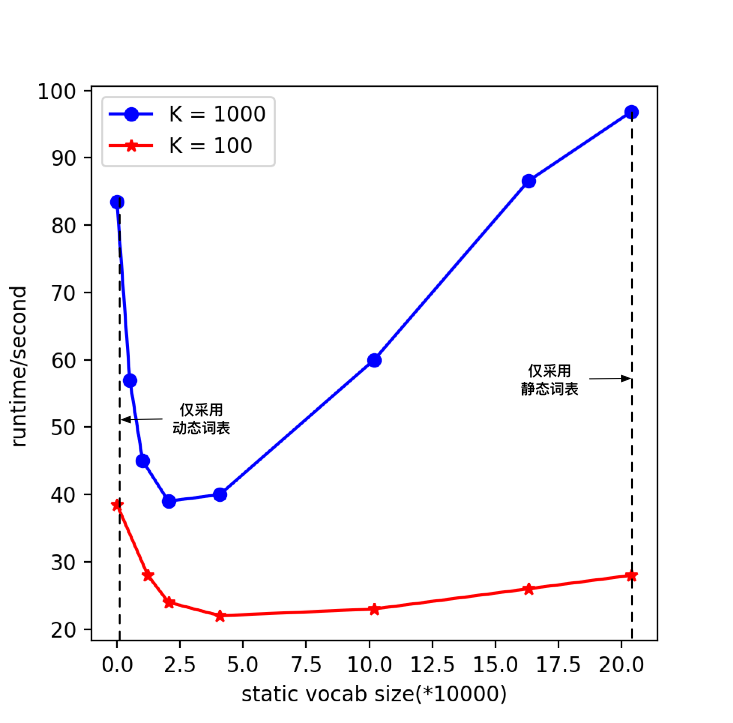
\includegraphics[height=0.41\linewidth]{static-vocab-vs-runtime}
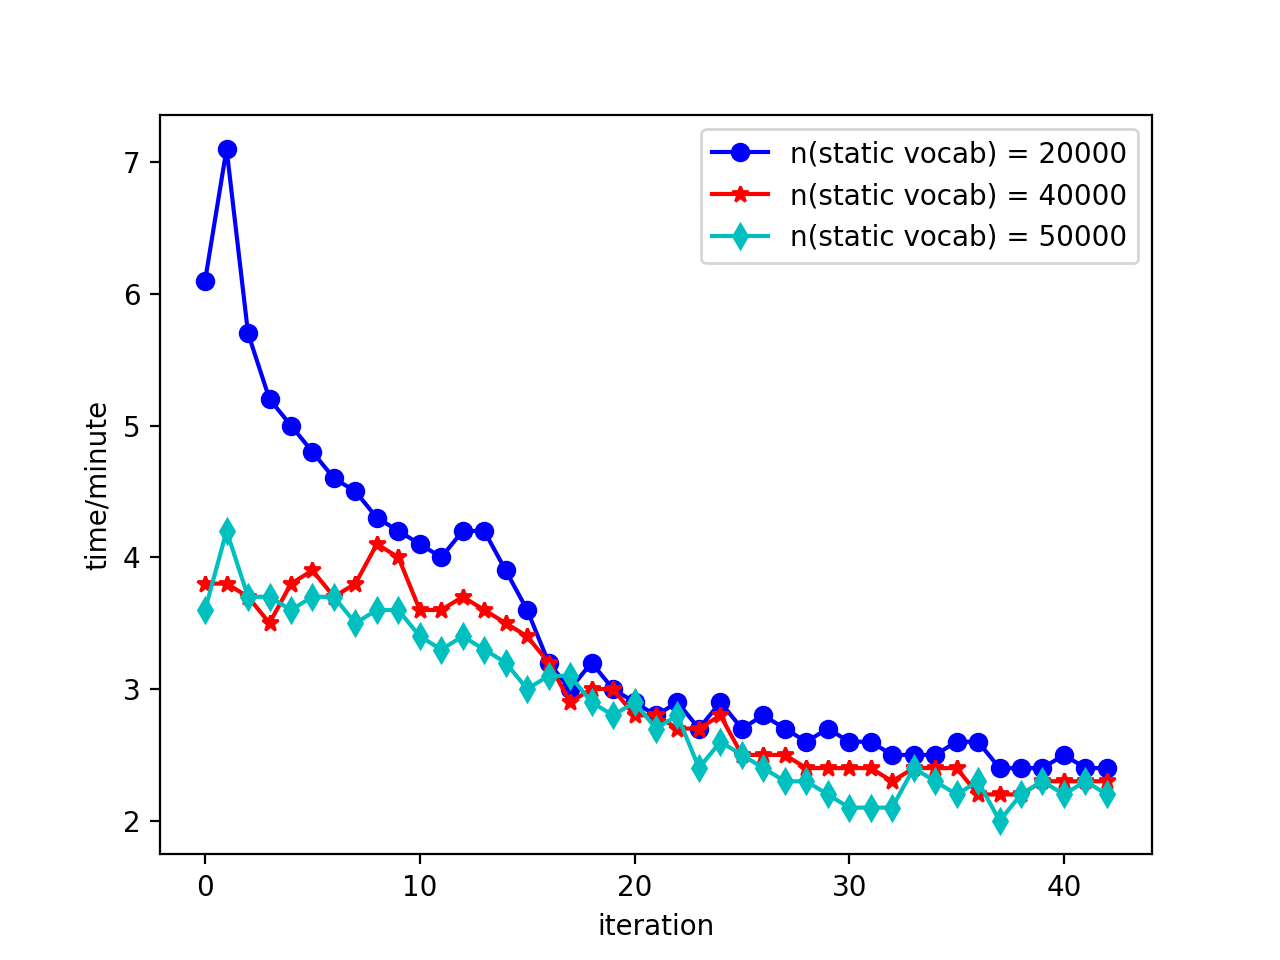
\includegraphics[height=0.41\linewidth]{static-vocab-runtime-iteration}
\caption{静态词表大小与运行时间关系示意}
\label{fig:static-vocab-runtime}       % Give a unique label
\end{figure}

图\ref{fig:static-vocab-runtime}所显示的是静态词表大小与算法运行时间之间的关系。

在左子图中,实验中每轮迭代遍历41310个文档,语料中出现的词汇总量为203891。
左子图中显示的纵坐标运行时间为算法采样10轮的时间平均值(单位为秒),横坐标表示的静态词汇表的大小(*10000)。
本文分别统计了主题维度为100和1000两种情况下,算法运行时间与静态词汇表大小之间的关系。
如图所示,我们不难发现曲线呈对钩形状。在这个实验中静态词汇表的带下设置为50000左右比较合适。
静态词汇表太大,低频词会逐渐增多,意味着混合参数中的Dense(V,Z)表会变得越来越稀疏,因而会大大降低算法的性能。
另外一方面静态词汇表也不能太小,语料中高频词的覆盖率占了绝大多数,小的静态词汇表无法充分地覆盖语料,使得许多参数访问被转向Sparse(V,Z),从而也会降低算法的性能。

在右子图中,实验中每轮迭代遍历808301个文档,语料中出现的词汇总量为982101。
纵坐标表示每轮迭代的运行时间(单位为分钟),横坐标表示算法的迭代轮数。
如果所示,本文分别设置了三组静态词表大小(20000,40000,50000),主题模型的维度都为1000。
不管静态词表的大小如何,随着迭代轮数的增长,运行时间都表现出下降的趋势。
起初三组实验算法运行时间存在明显的差异,其中静态词汇表大小为20000的实验显示运行时间远大于另外两组。
但是随着时间的推移,运行时间逐渐降低并且逼近另外两组。这是因为Sparse(V, Z)随着算法迭代轮数的增加越来越稀疏,带来了网络传输量的急剧下降。

\subsection{算法的可用性实验}
\begin{figure}[htb]\centering
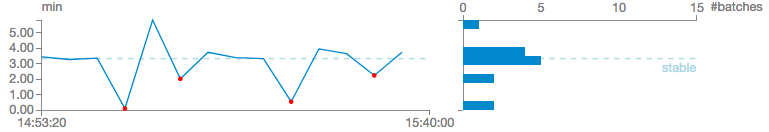
\includegraphics[width=1\linewidth]{stream-process-time}
\caption{Spark Streaming下流式主题模型的失败恢复实验}
\label{fig:stream-process-time}       % Give a unique label
\end{figure}
如上图所示,左子图为流式主题模型算法各批次运行时间图,右子图为运行时间的柱状图统计。
图\ref{fig:stream-process-time}中的虚线显示每个批次限定的合理运行时间为20000秒(3.3分钟)。
红色的点表示故障发生的时刻。可见故障发生后,算法重启具有一定的时延,但是都能够继续正常的运行。
通过左子图,我们还能够判断,除了少数超时和故障发生的情况,大部分时候算法维持稳定运行状态。
这得益于本文良好的算法设计。

\begin{figure}[htb]\centering
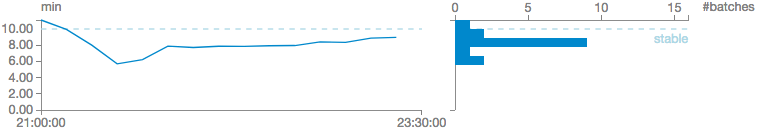
\includegraphics[width=1\linewidth]{stable-process}
\caption{流式主题模型运行状况示例}
\label{fig:stable-process}       % Give a unique label
\end{figure}

如图\ref{fig:stable-process}上图显示的是算法各个批次的运行时间,以及柱状统计图。
在参数设置合理的情况下,本文算能够持续鲁棒地运行。
在这个例子中,我们每个批次共输入50000篇文档,迭代15轮,主题个数为100,每个批次时间间隔10分钟。
我们发现除了算法开始执行的前几个批次算法运行时间超时外,其他批次的处理基本上不会超时。
并且,随着时间的推移每个批次的运行时间呈下降趋势,并最终稳定在8分钟左右。
这是因为在算法持续运行过程中,主题模型的参数逐渐变得稀疏,使得算法的运行效率有所提高。
并且当运行足够长时间之后,算法的稀疏性不会再有太大的变化。

\section{本章小结}
本章主要介绍了流式主题模型的参数结构设计。
在分布式并行算法实现中,人们通常会提及数据并行和模型并行两种并行方式。
参数服务器的出现,使得这两种并行方式能够更好地结合在一起。
在本文的算法实现中,我们应用了参数服务器作为分布式并行流式主题模型的主要组件。

在本章我们着重分析了流式数据环境下,动态增长的词汇表对主题模型实现所造成的影响。
并根据分析得到的结论提出了稠密和稀疏并存的参数数据结构。这种设计方案不仅有效地降低了参数存储的空间消耗,
还能够降低算法采样过程中的同步和更新所带来的网络消耗。

除了参数数据结构的设计,在本章中我们还介绍了,我们如何选择参数的数值类型和如何维护参数系数表Sparse(V, Z)的稀疏性。
在章节的最后,我们还指出了在流式环境下,算法系统因为多种原因所造成的失败。
为了保证算法系统的稳定性,本文提出了针对分布式流式主题模型的参数备份和恢复方案。
实验证明,本章提出的参数数据结构和容错机制能够保证算法高效和稳定运行。
